The Deployment Diagram shown below describes how the logical components designed in the context of the Component Diagram are to be physically deployed on the different devices needed for the functioning of the system.

As shown, the app server hosts the main logic components and manages their interaction. It provides access to them through the APIs defined in \autoref{sec:components_interfaces} and guarantees they can access the data layer residing on the database server.\newline
Every client with a significant application layer implements a limited subset of components responsible to interpret the inputs from the users and perform requests to the app server. When needed, an apposite module for the localization is included as well.\newline
The web server provides static web pages and the logic necessary to the browser to interact with the app server.

\begin{sidewaysfigure}
	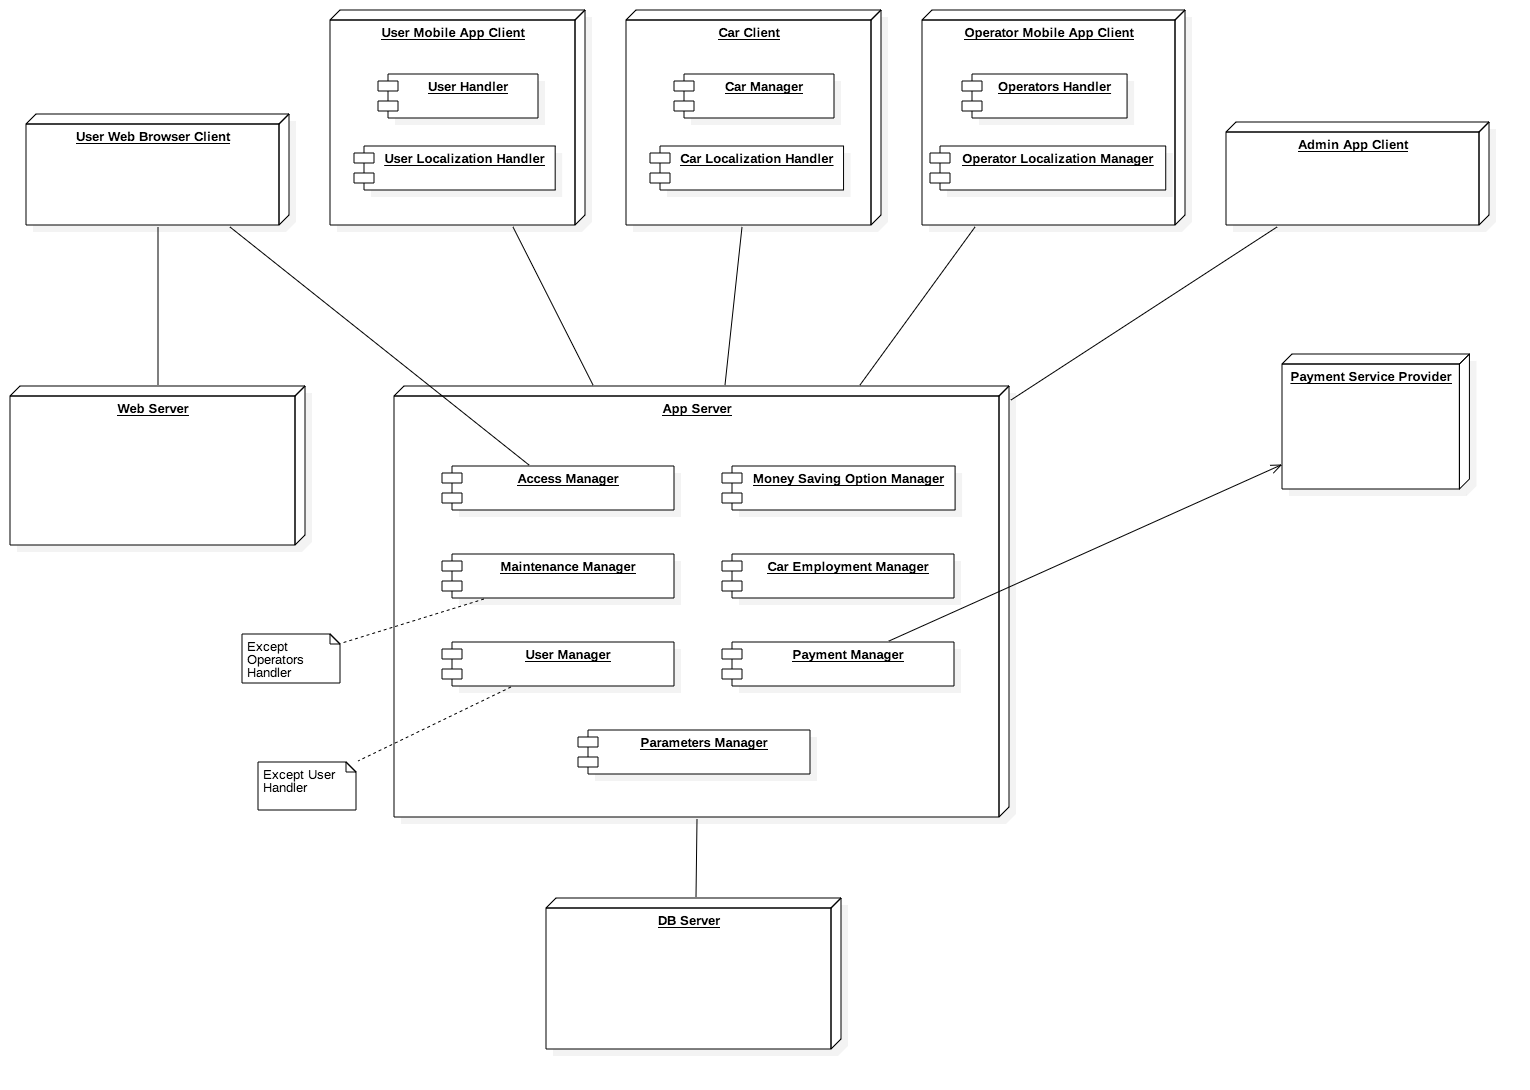
\includegraphics[width=\hsize, center]{img/deployment_diagrams/global.png}
\end{sidewaysfigure}

\subsubsection{Non-functional requirements choices}
	The architectural structure proposed addresses the non-functional requirements of \textit{integrity} and \textit{confidentiality} (see RASD) introducing a DMZ which separates with a firewall the app server, accessible from the outside network, from the database server. To avoid intrusions on the app server, another firewall is provided, with less restricting rules to allow outside clients to access. This way, even if an attack is performed to the app server, a more impenetrable layer of security still divides the intruders from the sensitive data. The structure just described is a standard pattern in the design of three-layer architectures.

	The app server is designed as a distributed system completely replicated in at least another physical machine, to fulfil the requirement of \textit{availabilty} and partially address the requirement of \textit{performance} (see RASD). A load balancer is expected to redirect the workload to the appropriate physical server. The number of servers can be increased in future if the workload requires it. This structure, along with a proper firewall configuration, helps to reduce the risk of failure for DOS attacks.

	Internally, each physical server is implemented following the \textit{elasticity pattern}, to fulfil the requirement of \textit{performance} (see RASD) while maintaining the number of allocated resources low. Thus, the components are to be instantiated according to the present load of clients' requests. An \textit{elastic load balancer} is used to manage the scaling process.

	To address the requirement of \textit{robustness} (see RASD) a simple error handling in the client application is enough. However, given the importance of failure management to avoid damages or theft to be performed to the cars, the data layer is chosen to be distributed.

	Lastly, the modularization of components and the possibility for the administrators to modify the core parameters of the system through the \textit{Parameters Manager} is conform to the \textit{design for flexibility} principle and satisfies the non-functional requirement of \textit{flexibility} (see RASD).
\FloatBarrier

\subsubsection{Technological choices}
	% TODO talk about technological choices for APIs, app server, db server, mobile apps, desktop apps, browser, ...
	From a technological point of view, the implementation of the system relies on the following choices.
	\begin{description}
		\item[User mobile app client.] The mobile app is to be developed with native technologies according to the mobile OS running on the device. In particular:
			\begin{itemize}
				\item[Android] Java for Android, with support for Android 4.4+.
				\item[iOS] Objective-C, with support for iOS 6+.
				\item[Windows Phone] C\#, with support for Windows 10 mobile.
			\end{itemize}
		The choice of covering the 3 most important OS on the market fulfils the \textit{design for portability} pattern. To address this pattern and be able to release the system in shorter time, some non-native options have been taken in consideration (e.g. Apache Cordova). However, this solutions showed to provide limited access to native functionalities such as the GPS system and the Bluetooth, which are instead very important for the system-to-be (i.e. localization, communication with the car). Therefore, native solutions have been preferred, to have full control of the device. This choice guarantees also a better user experience.

		\item[Operator mobile app client.] This internal application helps the operators to track their activity during the interventions. The company provides them with an Android tablet, so the application is to be compatible with it. Moreover, to provide more usability, this application is designed to be deployed on both tablet and smartphones, managing a responsive layout. The company choice of the Android platform addresses the need of inexpensive but efficient devices to run mainly the application. As for the \textit{User mobile app client}, the application is to be developed in native language (Java for Android, with support for Android 4.4+) to exploit some system-level functionalities.

		\item[Car client.] The system managing the whole car is running on the Android tablet installed. It is connected to the control unit of the car and communicates with the rest of the system though the APIs provided by the app server. It also exposes some APIs of its own, to be accessed by the app server (i.e. request of status information, sending of commands). Besides, a Bluetooth listener receives the requests from near users to unlock the car (if a reservation has been made.

		\item[Admin app client.] An internal desktop application is developed to provide access to the admin to the parameter manager and the operator dispatching area. To avoid restrictions in the future equipment of the admins, the application is planned to be developed in Java, ensuring portability on every desktop and laptop OS. In addition, given the configuration of the app server (see later), Java EE is required, to guarantee uniformity with the back-end system and simplify the development.

		\item[App server.] This server is to be developed using the Java EE platform. This framework will help to provide the elasticity required and simplify the connections with the database through JPA. The app server exposes the APIs required by the clients as RESTful web services.

		\item[Web server.] The web server simply hosts a very limited website with information about the service and an account management section. Given the simple functionalities, it is not worth the effort of building a Java EE system; instead, the most basic set of web technologies are to be used: HTML5, CSS3 and JS client-side and PHP7 server-side. The choice of PHP over other languages is due to the previous knowledge of the language by the team; in addition, it is a well spread language and can be easily maintained by other developers of the company in the future. For the account management section, the JS script communicates with the application server by means of AJAX calls to the web services.

		\item[Database server.] A distributed MySQL database, running on a set of Ubuntu servers, manages all the data needed by the application.
	\end{description}

% TODO provide physical diagram with distribution and platforms
